% ============================================================================
% Apresentação de Defesa de Mestrado
% Análise de Vibração Livre de Estruturas no Estado Plano
% através do Método dos Elementos Virtuais
%
% Autor: Vinícius Belmar Almeida Prado Pohl
% Orientador: Prof. Dr. Marcos Arndt
% PPGMNE / UFPR - 2026
%
% Template oficial da Universidade Federal do Paraná
% ============================================================================
\documentclass[aspectratio=169]{beamer}
\setbeamertemplate{footline}[frame number]
\usepackage[utf8]{inputenc}
\usepackage[T1]{fontenc}
\usepackage[brazil]{babel}
\usepackage{graphicx}
\usepackage{enumerate}
\usepackage{subcaption}
\usepackage{booktabs}
\usepackage{multirow}
\usepackage{hyperref}
\usepackage{makecell}
\usepackage{amsmath,amssymb,bm}
\usepackage{tikz}
\usetikzlibrary{positioning,arrows.meta,shapes.geometric}

\usetheme{default}
\usecolortheme{orchid}
\usefonttheme[onlymath]{serif}

\beamertemplatenavigationsymbolsempty
\hypersetup{pdfpagemode=FullScreen}

% --- Página de título personalizada ---
\makeatletter
\newcommand\titlegraphicii[1]{\def\inserttitlegraphicii{#1}}
\titlegraphicii{}
\setbeamertemplate{title page}
{
  \vbox{}
   {\usebeamercolor[fg]{titlegraphic}\inserttitlegraphic\hfill\inserttitlegraphicii\par}
  \begin{centering}
    \begin{beamercolorbox}[sep=2pt,center]{institute}
      \usebeamerfont{institute}\insertinstitute
    \end{beamercolorbox}
    \begin{beamercolorbox}[sep=12pt,center]{title}
      \usebeamerfont{title}\inserttitle\par%
      \ifx\insertsubtitle\@empty%
      \else%
        \vskip0.2em%
        {\usebeamerfont{subtitle}\usebeamercolor[fg]{subtitle}\insertsubtitle\par}%
      \fi%
    \end{beamercolorbox}%
    \vskip0.2em\par
    \begin{beamercolorbox}[sep=2pt,center]{author}
      \usebeamerfont{author}\insertauthor
    \end{beamercolorbox}
    \begin{beamercolorbox}[sep=4pt,center]{date}
      \usebeamerfont{date}\insertdate
    \end{beamercolorbox}%
  \end{centering}
}
\makeatother

% --- Metadados ---
\title{Análise de Vibração Livre de Estruturas no Estado Plano\\
através do Método dos Elementos Virtuais}
\author{\textbf{Vinícius Belmar Almeida Prado Pohl}}
\institute{UNIVERSIDADE FEDERAL DO PARANÁ \\
SETOR DE CIÊNCIAS EXATAS \\
PROGRAMA DE PÓS-GRADUAÇÃO EM MÉTODOS NUMÉRICOS EM ENGENHARIA}
\date{Orientador: Prof.\ Dr.\ Marcos Arndt \\[0.3em] Curitiba, 2026}

\AtBeginSubsection[]
{
  \begin{frame}<beamer>{Roteiro}
    \tableofcontents[currentsection,currentsubsection]
  \end{frame}
}

\begin{document}

%=============================================================================
% CAPA
%=============================================================================
{%
 \usebackgroundtemplate{%
  \centering
  
\includegraphics[width=\paperwidth]{CapaUFPR.png}%
 }
\begin{frame}
  \titlepage
\end{frame}
}

%=============================================================================
% ROTEIRO + CONTEÚDO (fundo contínuo)
%=============================================================================
{%
 \usebackgroundtemplate{%
  \centering
  
\includegraphics[width=\paperwidth]{FundoUFPR2.png}%
 }
\begin{frame}{Roteiro}
  \tableofcontents
\end{frame}

%=============================================================================
\section{Motivação, objetivos e contribuição}

\begin{frame}{Motivação}
  \begin{itemize}
      \item Análise dinâmica essencial para conforto e segurança (ressonância).
      \item Estruturas esbeltas elevam a importância das vibrações.
      \item MEF clássico: geometria restrita e sensível à distorção.
      \item Pré-processamento de malhas conformes é custoso.
      \item Necessidade de elementos de topologia arbitrária.
  \end{itemize}
\end{frame}

\begin{frame}{Contribuição}
  \begin{itemize}
      \item 1ª implementação de MEV no PPGMNE.
      \item Projetores generalizados para qualquer ordem de interpolação.
      \item Quatro tipologias estruturais práticas: Uma chapa engastada, uma chapa trapezoidal perfurada, uma barragem de terra e uma parede estrutural.
      \item Comparação sistemática MEF $\times$ MEFG $\times$ MEV
  \end{itemize}
  \begin{columns}[T]
    \begin{column}{0.48\textwidth}
      \centering
      \includegraphics[width=0.45\linewidth]{figuras/capítulo 5/placa quadrada/Placa engastada.png}
      \includegraphics[width=0.5\linewidth]{figuras/capítulo 5/placa com furo/5.1.png}
    \end{column}
    \begin{column}{0.48\textwidth}
      \centering
      \includegraphics[width=0.6\linewidth]{figuras/capítulo 5/Barragem/Captura de tela 2026-08-19 082612.png}
      \includegraphics[width=0.35\linewidth]{figuras/capítulo 5/parede estrutural/sheer wall.png}
    \end{column}
  \end{columns}
\end{frame}

\begin{frame}{Objetivos}
  \begin{block}{Objetivo geral}
    Investigar e implementar a formulação do MEV para a solução do problema
    de autovalores generalizados associado à análise de vibração livre de
    estruturas em estado plano.
  \end{block}

  \vspace{0.3em}
  \textbf{Objetivos específicos}
  \begin{itemize}
    \item Desenvolver a formulação do MEV em soluções lineares e de alta ordem ($k=1$ e $k=2$).
    \item Implementar o MEV para análise de vibração livre e validar com modelos de referência.
    \item Comparar os resultados obtidos pelo MEV com as soluções do MEF e do MEFG.
  \end{itemize}
\end{frame}

%=============================================================================
\section{Revisão e posicionamento}

\begin{frame}{Desenvolvimento do MEV}
  \begin{itemize}
    \item Origem no Método das Diferenças Finitas Miméticas (MFDM).
    \item Formalização por Beirão da Veiga et al.\ (2013) --- equação de Poisson.
    \item Extensão para campos vetoriais e elasticidade linear (Da Veiga et al., 2013).
    \item Introdução do projetor $L^2$ (Ahmad et al., 2013) e formulações generalizadas.
    \item Evolução: ordem superior, contornos curvos, formulações não conformes e mistas.
  \end{itemize}
\end{frame}

\begin{frame}{MEV em elasticidade e dinâmica --- lacuna}
  \begin{columns}[T]
    \begin{column}{0.48\textwidth}
      \textbf{Elasticidade}
      \begin{itemize}
        \item Linear e quase-incompressível
        \item Pequenas e grandes deformações
        \item Elastoplasticidade
        \item Formulações mistas
      \end{itemize}
    \end{column}
    \begin{column}{0.48\textwidth}
      \textbf{Dinâmica}
      \begin{itemize}
        \item Equações parabólicas e hiperbólicas
        \item Elastodinâmica
        \item Integração explícita/implícita
        \item Vibração de placas Kirchhoff-Love
      \end{itemize}
    \end{column}
  \end{columns}

  \vspace{0.7em}
  \begin{alertblock}{Lacuna identificada}
    Há escassez de estudos do MEV aplicado à análise dinâmica de estruturas. 
  \end{alertblock}
\end{frame}

%=============================================================================
\section{Fundamentos}

\begin{frame}{Equação diferencial do problema}
  Forma forte da elastodinâmica em $\Omega\times(0,T]$:
  \begin{align*}
    \rho\,\ddot{u} - \nabla\cdot\sigma(u) &= f && \text{em }\Omega\times(0,T], \\
    u &= g_D && \text{em }\Gamma_D\times(0,T], \\
    \sigma(u)\,n &= g_N && \text{em }\Gamma_N\times(0,T], \\
    u &= u_0 && \text{em }\Omega\times\{0\}, \\
    \dot{u} &= u_1 && \text{em }\Omega\times\{0\}.
  \end{align*}
\end{frame}

\begin{frame}{Formulação variacional}
  Problema variacional: encontrar $w(t)\in\mathbb{V}:=H^1(\Omega)$ tal que
  \[
    m(\ddot{w},v) + a(w,v) = \tilde{L}(v,t)
    \qquad\forall v\in\mathbb{V}.
  \]

  Explicitamente:
  \[
    \int_\Omega\rho\,\ddot{u}\cdot v\,dx
    + \int_\Omega\mathbb{C}\,\epsilon (u) \cdot \epsilon (v)\,dx
    = \int_\Omega f\cdot v\,dx
    + \int_{\Gamma_N}g_N\cdot v\,dS.
  \]

  \vspace{0.3em}
  Vibração livre não amortecida ($f=0$, $g_N=0$) $\Rightarrow$
  problema de autovalores generalizado:
  \[
    \mathbf{K}\boldsymbol{\phi} = \omega^2\mathbf{M}\boldsymbol{\phi}.
  \]
\end{frame}


\begin{frame}{O elemento virtual}
  \begin{columns}[T]
    \begin{column}{0.45\textwidth}
      \begin{itemize}
        \item Discretização direta no domínio físico; elementos com formato e nº de nós \textbf{arbitrários}.
        \item A função virtual \textbf{não precisa ser conhecida explicitamente} no interior.
        \item Solução computável obtida por \textbf{projetores polinomiais}.
        \item Graus de liberdade são: Nós de vértice, $k-1$ nós internos por aresta, $n_{k-2}$ momentos internos por elemento.
      \end{itemize}
    \end{column}
    \begin{column}{0.52\textwidth}
      \centering
      \includegraphics[width=\linewidth]{figuras/capítulo 4/4.4.png}
    \end{column}
  \end{columns}
\end{frame}

\begin{frame}{Espaços virtuais $V_k$ e $W_k$}
  \begin{block}{Espaço virtual $V_k(\Omega_v)$}
    \[
      V_k(\Omega_v)=\bigl\{
        v\in H^1(\Omega_v):\;
        v|_{\partial\Omega_v}\in \mathbb{P}_k(\partial\Omega_v),\;
        \Delta v\in\mathbb{P}_{k-2}(\Omega_v)
      \bigr\}
    \]
    Para $k=1$: funções internas harmônicas ($\Delta v=0$).
  \end{block}

  \vspace{0.35em}
  \begin{block}{Espaço ampliado $W_k(\Omega_v)$ (projetor $L^2$)}
    \begin{align*}
      W_k(\Omega_v) = \bigl\{ v\in H^1(\Omega_v) : \;& v|_{\partial\Omega_v}\in \mathbb{P}_k(\partial\Omega_v),\; \Delta v \in\mathbb{P}_{k}(\Omega_v), \\
      & a(\mu,v)=0\;\forall\mu\in\mathbb{P}_k\backslash\mathbb{P}_{k-2}(\Omega_v) \bigr\}
    \end{align*}

    Aumenta o grau do laplaciano interno $\Rightarrow$ permite computar $\Pi_k^0$ de forma estável.
  \end{block}
\end{frame}

\begin{frame}{Decomposição das matrizes de rigidez e massa}
  \textbf{Decomposição das matrizes elementares:}
  \[
    \mathbf{K}^E = \mathbf{K}_{\mathrm{cons}}^E + \mathbf{K}_{\mathrm{stab}}^E,
    \qquad
    \mathbf{M}^E = \mathbf{M}_{\mathrm{cons}}^E + \mathbf{M}_{\mathrm{stab}}^E.
  \]  
  \begin{columns}[T]
    \begin{column}{0.48\textwidth}
      \textbf{Consistência}
      \[
        \mathbf{K}_{\mathrm{cons}}^E  = a_h^E(\Pi,\Pi)\quad\forall\, \Pi \in[\mathbb{P}_k]^d,
      \]

      \[ \mathbf{M}_{\mathrm{cons}}^E  = a_h^E(\Pi,\Pi)\quad\forall\, \Pi \in[\mathbb{P}_k]^d,
      \]
    \end{column}
    \begin{column}{0.48\textwidth}
      \textbf{Estabilidade}
      \[
        \mathbf{K}_{\mathrm{stab}}^E = \tau_K\,
        (\mathbf{I}-\boldsymbol{\Pi})^\top
        (\mathbf{I}-\boldsymbol{\Pi})
      \]

      \[\mathbf{M}_{\mathrm{stab}}^E = \tau_m\,
        (\mathbf{I}-\boldsymbol{\Pi})^\top
        (\mathbf{I}-\boldsymbol{\Pi})
      \]
    \end{column}
  \end{columns}  
  \begin{block}{Propriedades de consistência e estabilidade}
      \[
        a^E(p,v) = a_h^E(p,v)
        \quad\forall\, \Pi \in[\mathbb{P}_k]^d
      \]  \[
        \alpha_*\, a^E(v,v) \leq
        a_h^E(v,v) \leq
        \alpha^*\, a^E(v,v)
      \]
  \end{block}
\end{frame}

\begin{frame}{Projetores e decomposição da função virtual}
  A função virtual $\varphi \in V_k$ é decomposta em: $\varphi = \Pi_k \varphi + (\varphi - \Pi_k \varphi)$
  \textbf{Projetores} (computáveis só com os gl do elemento):
  \vspace{1em}
  \begin{itemize}
    \item $\Pi_k^\nabla$ --- projeção elíptica ($H^1$) $\rightarrow$ \textbf{rigidez}
    \item $\Pi_k^0$ --- projeção $L^2$ $\rightarrow$ \textbf{massa}
    \item $\Pi_{k-1}^\varepsilon$ --- projeção das deformações
  \end{itemize}
  \vspace{2em}
  \centering
  $a_h^E(\Pi \varphi, (\varphi - \Pi \varphi)) = 0 \quad m_h^E(\Pi \varphi, (\varphi - \Pi \varphi)) = 0$
\end{frame}

\begin{frame}{Tipos de estabilização}
  \[ \tau \,(\mathbf{I}-\mathbf{D}\boldsymbol{\Pi}^0)^\top
      (\mathbf{I}-\mathbf{D}\boldsymbol{\Pi}^0),
    \qquad \tau \,(I - D (D^T D)^{-1} D^T)
  \]

  \vspace{0.15em}
  \textbf{Escolhas de $\tau_K$:}
  \begin{align*}
    \tau_K &= \max_i(K^C_{ii})
      && \text{(uniforme)} \\[0.15em]
    \tau_K &= \max(2\mu,\lambda)
      && \text{(físico / Lamé)} \\[0.15em]
    \tau_K &= \alpha_0\,\mathrm{tr}(K^C)
      && \text{(traço; $\alpha_0\!\approx\!0{,}5$)} \\[0.15em]
    \tau_K &= \mathrm{diag}\bigl(|K^C_{ii}|\bigr)
      && \text{(D-Recipe)} \\[0.15em]
    \tau_K &= \max\!\Bigl(K^C_{ii},\;
      \alpha_0\,\tfrac{\mathrm{tr}(\mathbb{C})}{n_C}\Bigr)
      && \text{(D-Recipe híbrido)}
  \end{align*}

  \textbf{Escolhas de $\tau_m$:}
  \[
    \tau_m = \rho\,|\Omega_v|
    \qquad\text{ou}\qquad
    \tau_m = \rho\,h_E^2
  \]
\end{frame}


\begin{frame}{Métricas de desempenho}
  \begin{itemize}
    \item Erro relativo por modo:
      $e_{\mathrm{rel}} = \bigl|\frac{\omega-\tilde{\omega}}{\omega}\bigr|$
    \item MAPE --- erro percentual médio absoluto
    \item NRMSE --- raiz do erro quadrático médio normalizado
    \item MG --- média geométrica (índice composto)
    \item CAD --- coeficiente de acurácia de discretização
    \item GPR --- ganho de precisão relativo ao MEF
    \item CA --- coeficiente de acurácia em relação ao MEFG
  \end{itemize}
\end{frame}

%=============================================================================
\section{Casos de estudo}

% ----- Caso 1 -----
\begin{frame}{Caso 1 --- Chapa engastada: setup}
  \begin{columns}[T]
    \begin{column}{0.48\textwidth}
      \begin{itemize}
        \item $E=2{,}1\times10^{11}$, $\nu=0{,}3$, $\rho=8000$
        \item $1\times1\,\mathrm{m}$, $d=0{,}05\,\mathrm{m}$
        \item Borda esquerda engastada
        \item Malhas: CU4 / CU16 / CU64
        \item 5 técnicas de estabilização
        \item Ref.: Torii (2012), MEFH $p=9$
      \end{itemize}
    \end{column}
    \begin{column}{0.50\textwidth}
      \centering
      \includegraphics[width=0.7\linewidth]{figuras/capítulo 5/placa quadrada/malha uniforme.png}
    \end{column}
  \end{columns}
\end{frame}

\begin{frame}{Caso 1 --- Refino e estabilização}
  \begin{columns}[T]
    \begin{column}{0.37\textwidth}
      \centering
      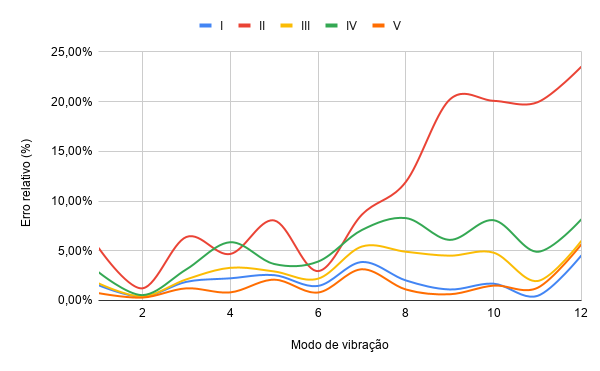
\includegraphics[width=\linewidth]{figuras/Capítulo 5/Placa quadrada/Erro absoluto x Modo de vibração (Malha de 64 elementos).png}
      \vspace{1.0em}
      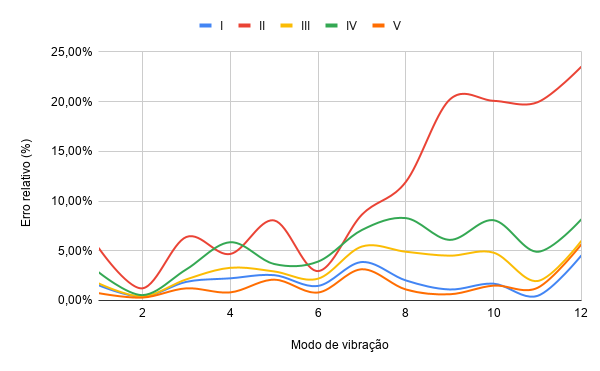
\includegraphics[width=\linewidth]{figuras/Capítulo 5/Placa quadrada/Erro absoluto x Modo de vibração (Malha de 64 elementos).png}
    \end{column}
    \begin{column}{0.37\textwidth}
      \centering
      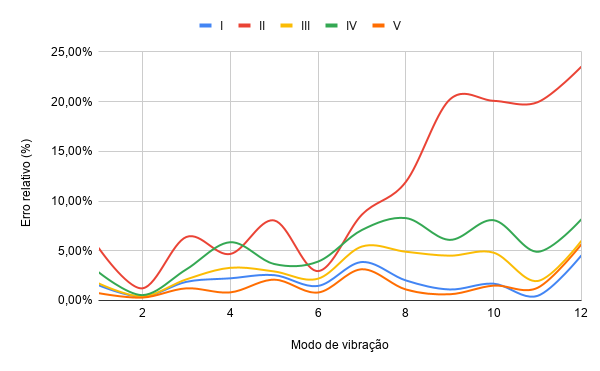
\includegraphics[width=\linewidth]{figuras/Capítulo 5/Placa quadrada/Erro absoluto x Modo de vibração (Malha de 64 elementos).png}
      \vspace{1.0em}
      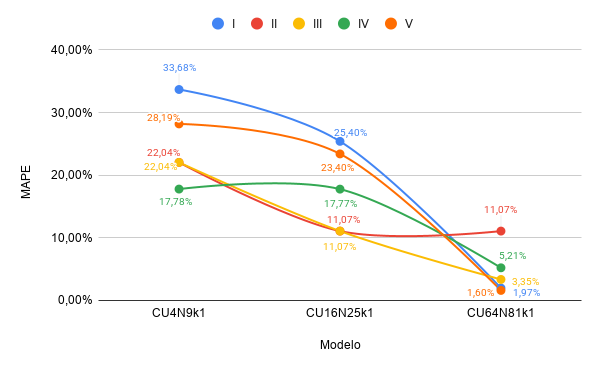
\includegraphics[width=\linewidth]{figuras/Capítulo 5/Placa quadrada/MAPE x Malha.png}
    \end{column}
    \begin{column}{0.25\textwidth}
      \begin{enumerate}[I.]
        \item $\tau_K = \max_i(K^C_{ii})$ 
        \item $\tau_K = \max(2\mu,\lambda)$ 
        \item $\tau_K = \alpha_0\,\mathrm{tr}(K^C)$ 
        \item $\tau_K = \mathrm{diag}\bigl(|K^C_{ii}|\bigr)$ 
        \item $\tau_K = \max\!\Bigl(K^C_{ii},\; \alpha_0\,\tfrac{\mathrm{tr}(\mathbb{C})}{n_C}\Bigr)$
      \end{enumerate}
    \end{column}
  \end{columns}
  \vspace{0.3em}
  \footnotesize
  \textbf{Todas as estabilizações convergem com $h$; a melhor em malha grossa \textit{não} é necessariamente a melhor em malha fina.}
\end{frame}

\begin{frame}{Caso 1 --- Malhas distorcidas}
  \begin{columns}[T]
    \begin{column}{0.48\textwidth}
      \centering
      \includegraphics[width=0.7\linewidth]{figuras/capítulo 5/placa quadrada/malha distorcida.png}
    \end{column}
    \begin{column}{0.48\textwidth}
      \centering
      \includegraphics[width=0.7\linewidth]{figuras/capítulo 5/placa quadrada/malha distorcida.png}
    \end{column}
  \end{columns}
  \vspace{0.3em}
  \centering
  \footnotesize
  Malhas distorcida e severamente distorcida (CD e CSD) com 4 elementos.
\end{frame}

\begin{frame}{Caso 1 --- Distorção e modos}
  \begin{columns}[T]
    \begin{column}{0.48\textwidth}
      \centering
      \includegraphics[width=0.7\linewidth]{figuras/capítulo 5/placa quadrada/MAPE x Malha - Comparação de refino e distorção.png}
    \end{column}
    \begin{column}{0.48\textwidth}
      \centering
      \includegraphics[width=0.7\linewidth]{figuras/capítulo 5/placa quadrada/Erro relativo X Modo de vibração - Estudo de distorção.png}
    \end{column}
  \end{columns}
  \vspace{1.0em}
  \centering
  \includegraphics[width=0.4\linewidth]{figuras/capítulo 5/placa quadrada/Erro relativo x Modo de vibração - Comparação entre métodos.png}
\end{frame}

% ----- Caso 2 -----
\begin{frame}{Caso 2 --- Chapa com furo: setup}
  \begin{columns}[T]
    \begin{column}{0.48\textwidth}
      \begin{itemize}
        \item Trapézio $10\times10$ + furo circular
        \item Zhao \& Steven (1996); Cittadin (2020)
        \item Malha base: \textbf{8} polígonos
        \item Nós extras no contorno do furo
        \item $k=1$ fixo (só aumenta GLs de borda)
      \end{itemize}
    \end{column}
    \begin{column}{0.50\textwidth}
      \centering
      \includegraphics[width=\linewidth]{figuras/capítulo 5/placa com furo/5.1.png}
    \end{column}
  \end{columns}
\end{frame}

\begin{frame}{Caso 2 --- Condicionamento e frequências}
  \begin{columns}[T]
    \begin{column}{0.48\textwidth}
      \centering
      \includegraphics[width=1.2\linewidth]{figuras/capítulo 5/placa com furo/Comparação de frequências com modos de vibração - Placa engastada com furo.png}
    \end{column}
    \begin{column}{0.48\textwidth}
      \centering
      \includegraphics[width=0.7\linewidth]{figuras/capítulo 5/placa com furo/Condicionamento de K por malha.png}
      \vspace{1.0em}
      \includegraphics[width=0.7\linewidth]{figuras/capítulo 5/placa com furo/Condicionamento de M.png}
    \end{column}
  \end{columns}
  \vspace{0.25em}
  \footnotesize
  8 elem.: MG $\approx 12{,}7\%$\;·\;
  32 elem.: MG $\approx 16{,}8\%$\;·\;
  64 elem.: MG $\approx 40{,}9\%$ ($\kappa(\mathbf{K})>6\times10^4$).
\end{frame}

\begin{frame}{Erros e CA}
  \begin{columns}[T]
    \begin{column}{0.48\textwidth}
      \centering
      \includegraphics[width=\linewidth]{figuras/capítulo 5/placa com furo/Curva de erros - Placa engastada com furo.png}
    \end{column}
    \begin{column}{0.48\textwidth}
      \centering
      \includegraphics[width=\linewidth]{figuras/capítulo 5/placa com furo/Erros relativos.png}
    \end{column}
  \end{columns}
  \vspace{1em}
  \footnotesize Valores de CA:
  17 gl: MG $0,72$\;·\;
  33 gl: MG $0,75$\;·\;
  45 gl: MG $0,71$\;·\;
  104 gl: MG $0,24$ 
\end{frame}

% ----- Caso 3 -----
\begin{frame}{Caso 3 --- Barragem de terra: setup}
  \begin{columns}[T]
    \begin{column}{0.48\textwidth}
      \begin{itemize}
        \item Estado plano de deformações
        \item Clough \& Chopra (1966)
        \item $H=91{,}44\,\mathrm{m}$, base $2\times137{,}2\,\mathrm{m}$
        \item Poucos elementos + muitos GLs
        \item Refino-$p$: $k=1\to k=2$
      \end{itemize}
    \end{column}
    \begin{column}{0.50\textwidth}
      \centering
      \includegraphics[width=\linewidth]{figuras/capítulo 5/barragem/Captura de tela 2026-08-19 082531.png}
      \vspace{4em}
      \includegraphics[width=\linewidth]{figuras/capítulo 5/barragem/Captura de tela 2026-08-19 082553.png}
    \end{column}
  \end{columns}
\end{frame}

\begin{frame}{Caso 3 --- Ordem polinomial}
  \begin{columns}[T]
    \begin{column}{0.48\textwidth}
      \centering
      \includegraphics[width=\linewidth]{figuras/capítulo 5/barragem/erro relativo k1.png}
    \end{column}
    \begin{column}{0.48\textwidth}
      \centering
      \includegraphics[width=\linewidth]{figuras/capítulo 5/barragem/Erro relativo k2.png}
    \end{column}
  \end{columns}
\end{frame}

\begin{frame}{Caso 3 --- Número de condicionamento}
  \begin{columns}[T]
    \begin{column}{0.48\textwidth}
      \centering
      \includegraphics[width=\linewidth]{figuras/capítulo 5/barragem/Condicionamento de K - Barragem de terra.png}
    \end{column}
    \begin{column}{0.48\textwidth}
      \centering
      \includegraphics[width=\linewidth]{figuras/capítulo 5/barragem/Condicionamento de M - Barragem de terra.png}
    \end{column}
  \end{columns}
\end{frame}

\begin{frame}{Caso 3 --- Comparação de erros globais}
  \begin{table}[htbp]
        \centering
        \caption{Avaliações globais dos erros dos modelos.}
        \small % Reduz o tamanho da fonte para o padrão acadêmico
        \begin{tabular}{lccccc}
            \toprule
            \multirow{2}{*}{\textbf{Modelo}} & \textbf{MEF} & \multicolumn{3}{c}{\textbf{8 elem.}} & \textbf{35 elem.} \\
            \cmidrule(lr){3-5} \cmidrule(lr){6-6}
            & \textbf{(14 gl)} & \textbf{(14 gl)} & \textbf{(30 gl)} & \textbf{(72 gl)} & \textbf{(94 gl)} \\
            \midrule
            MAPE  & 43,82\% & 39,96\% & 32,99\% & 11,08\% & 19,47\% \\
            NRMSE & 58,86\% & 48,40\% & 39,32\% & 13,98\% & 27,08\% \\
            MG    & 50,79\% & 43,98\% & 36,02\% & 12,44\% & 22,96\% \\
            \bottomrule
        \end{tabular}
      \end{table}
      \begin{table}[htbp]
        \centering
        \caption{Avaliações globais dos erros dos modelos para $k=2$.}
        \small % Reduz o tamanho da fonte para o padrão acadêmico
        \begin{tabular}{lcccc}
            \toprule
            \multirow{2}{*}{\textbf{Modelo}} & \multicolumn{3}{c}{\textbf{8 elem.}} & \textbf{35 elem.} \\
            \cmidrule(lr){2-4} \cmidrule(lr){5-5}
            & \textbf{(32 gl)} & \textbf{(64 gl)} & \textbf{(188 gl)} & \textbf{(256 gl)} \\
            \midrule
            MAPE  & 94,14\% & 62,23\% & 14,03\% & 4,13\% \\
            NRMSE & 90,33\% & 60,32\% & 12,97\% & 5,45\% \\
            MG    & 92,22\% & 61,27\% & 13,49\% & 4,75\% \\
            \bottomrule
        \end{tabular}
      \end{table}
\end{frame}

% ----- Caso 4 -----
\begin{frame}{Caso 4 --- Parede estrutural: setup}
  \begin{columns}[T]
    \begin{column}{0.48\textwidth}
      \begin{itemize}
        \item 4 pavimentos + aberturas (EPT)
        \item Nguyen-Thanh et al.\ (2010); Custódio (2022)
        \item Refino-h e estudo do comportamento ao refino.
        \item Quantidade de elementos é maior do que a quantidade de nós.
      \end{itemize}
    \end{column}
    \begin{column}{0.50\textwidth}
      \centering
      \begin{figure}[H]
    \centering
    \label{fig:5.24}
    \begin{subfigure}[htpb]{0.45\textwidth}
        \centering
        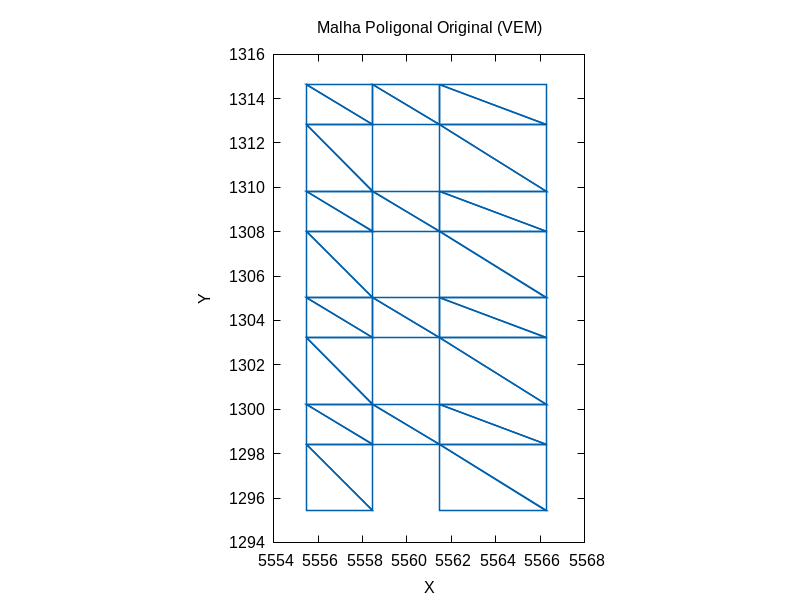
\includegraphics[width=\textwidth]{figuras/Capítulo 5/Parede estrutural/mesh_original 40.png}
        \label{fig:5.24a}
    \end{subfigure}
    \begin{subfigure}[htpb]{0.45\textwidth}
        \centering
        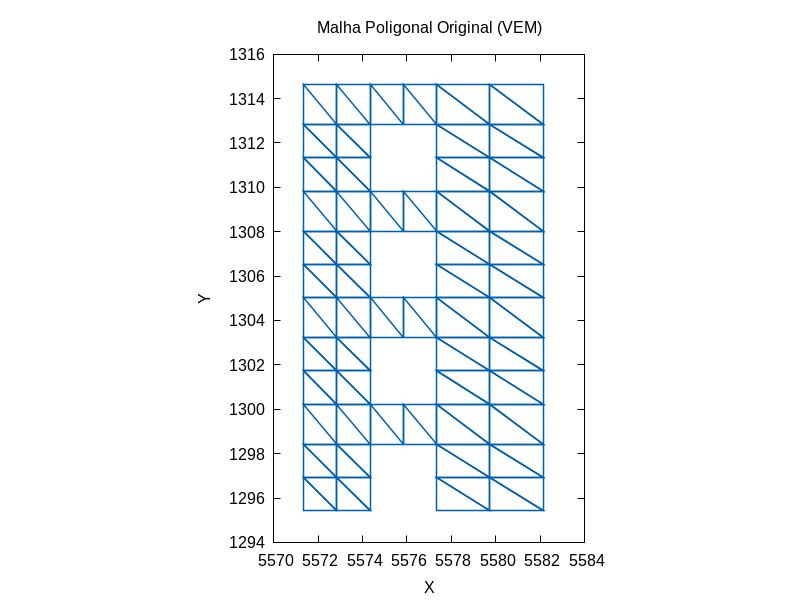
\includegraphics[width=\textwidth]{figuras/Capítulo 5/Parede estrutural/mesh_original 112.png}
        \label{fig:5.24b}
    \end{subfigure}
    \vspace{2mm}
    \begin{subfigure}[htpbb]{0.45\textwidth}
        \centering
        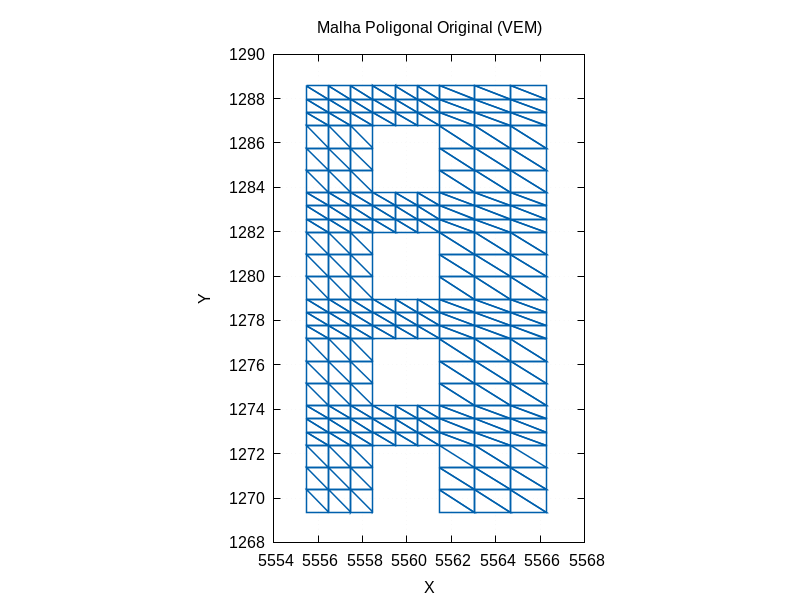
\includegraphics[width=\textwidth]{figuras/Capítulo 5/Parede estrutural/mesh_original 360.png}
        \label{fig:5.24c}
    \end{subfigure}
    \begin{subfigure}[htpb]{0.45\textwidth}
        \centering
        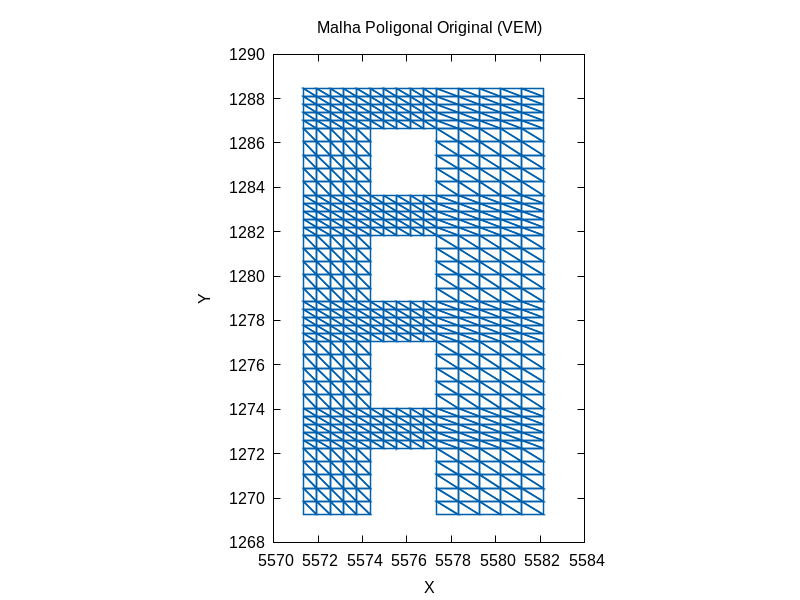
\includegraphics[width=\textwidth]{figuras/Capítulo 5/Parede estrutural/mesh_original 1000.png}
        \label{fig:5.24d}
    \end{subfigure}
\end{figure}  
    \end{column}
  \end{columns}
\end{frame}

\begin{frame}{Caso 4 --- Frequências e travamento de cisalhamento}
  \begin{columns}[T]
    \begin{column}{0.48\textwidth}
      \centering
      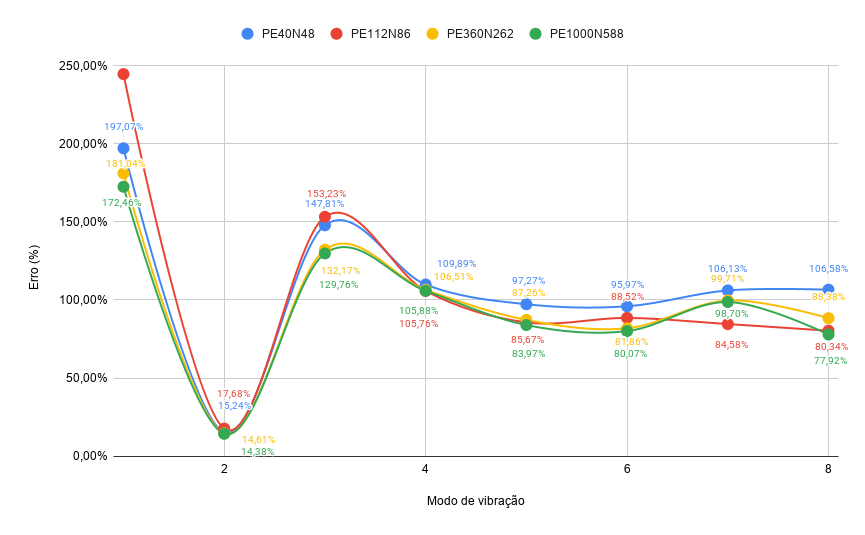
\includegraphics[width=\linewidth]{figuras/Capítulo 5/Parede estrutural/Erros relativos k1.png}
    \end{column}
    \begin{column}{0.50\textwidth}
      \centering
      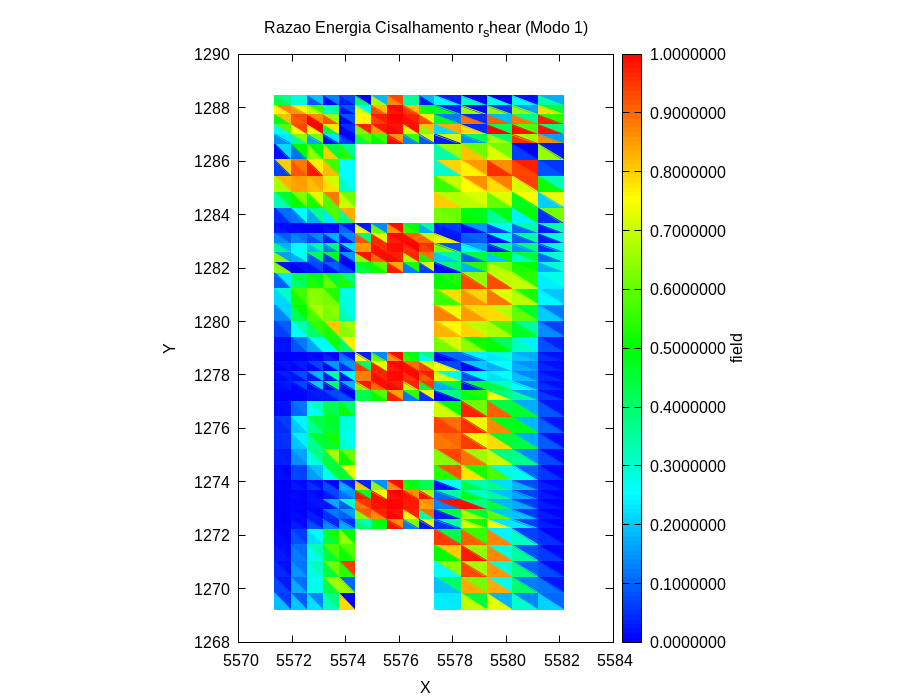
\includegraphics[width=0.7\linewidth]{figuras/Capítulo 5/Parede estrutural/locking_rshear_mode1 PE1000N588.png}
      \vspace{5mm}
      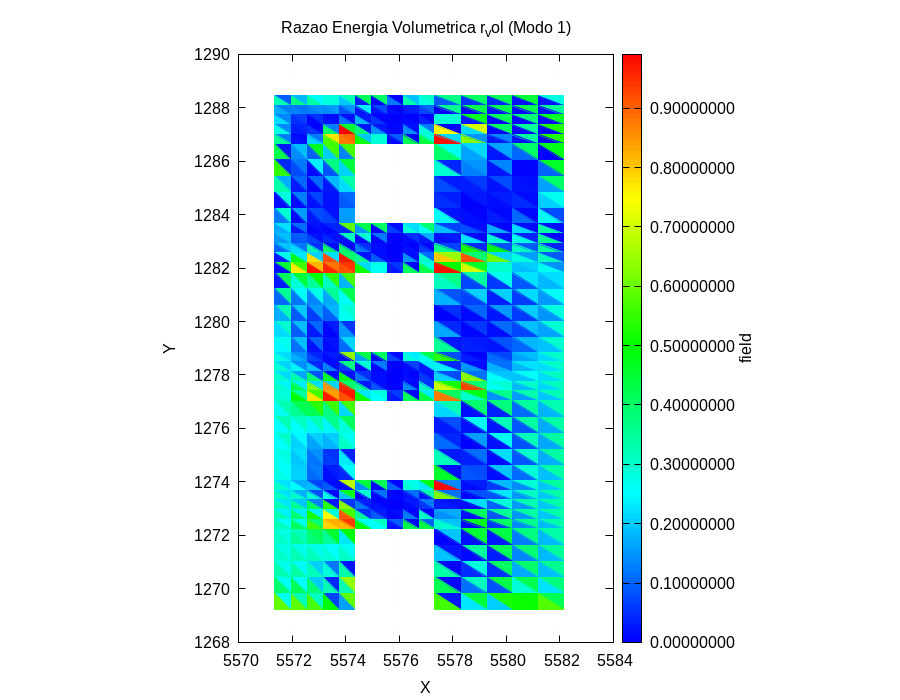
\includegraphics[width=0.7\linewidth]{figuras/Capítulo 5/Parede estrutural/locking_rvol_mode1 PE1000N588.png}
    \end{column}
  \end{columns}
\end{frame}

\begin{frame}{Estabilização da massa com $k=2$}
  \begin{columns}[T]
    \begin{column}{0.48\textwidth}
      \centering
      \includegraphics[width=\linewidth]{figuras/capítulo 5/parede estrutural/Erros relativos k2.png}
    \end{column}
    \begin{column}{0.48\textwidth}
      \centering
      \includegraphics[width=\linewidth]{figuras/capítulo 5/parede estrutural/erros relativos k2-2.png}
    \end{column}
  \end{columns}
\end{frame}

\begin{frame}{Caso 4 --- Deformadas}
  \begin{columns}[T]
    \begin{column}{0.48\textwidth}
      \centering
      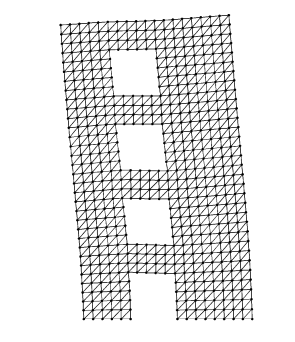
\includegraphics[width=0.5\linewidth]{figuras/Capítulo 5/Parede estrutural/Captura de tela 2026-09-16 084739.png}
      
      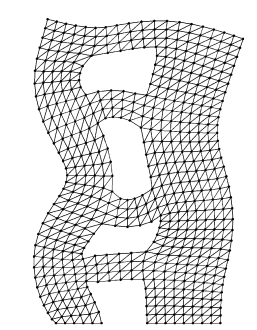
\includegraphics[width=0.45\linewidth]{figuras/Capítulo 5/Parede estrutural/Captura de tela 2026-09-16 084801.png}
    \end{column}
    \begin{column}{0.48\textwidth}
      \centering
      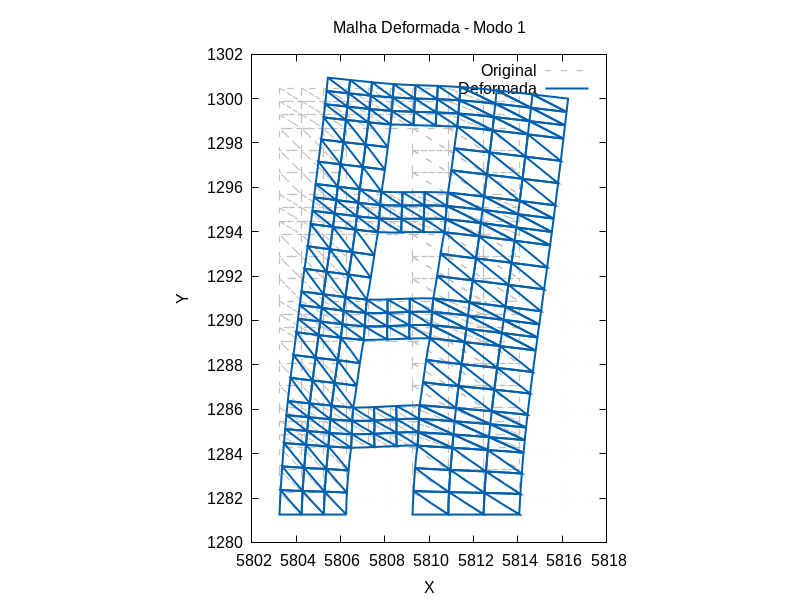
\includegraphics[width=0.7\linewidth]{figuras/Capítulo 5/Parede estrutural/deformed_mode_1.png}
      \vspace{5mm}
      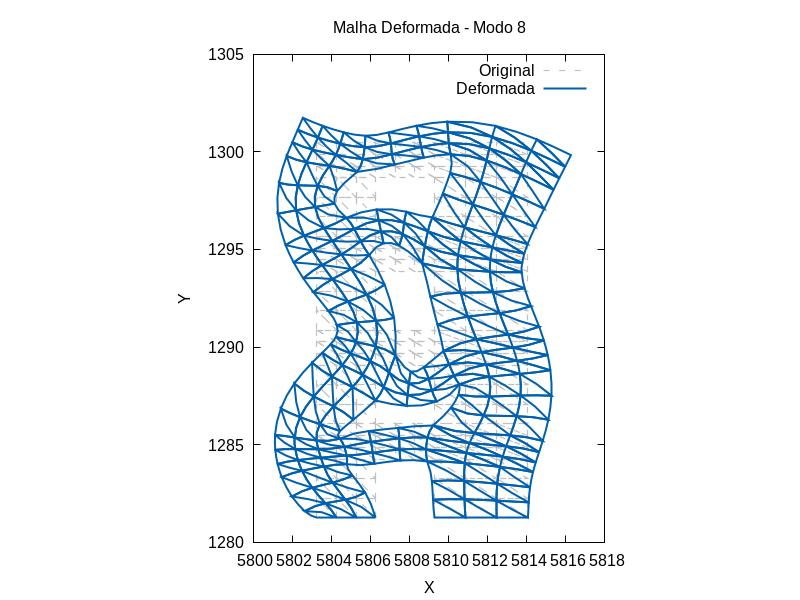
\includegraphics[width=0.8\linewidth]{figuras/Capítulo 5/Parede estrutural/deformed_mode_8.png}
    \end{column}
  \end{columns}
\end{frame}

\begin{frame}{Caso 4 --- Comparação com MEF-T6 e MEFG}
  \centering
  \begin{table}[htbp]
    \centering
    \caption{Comparação de erros do MEV com o MEF-T6 e MEFG.}
    \small % Reduz o tamanho da fonte para o padrão acadêmico
    \begin{tabular}{lccccc}
        \toprule
        \textbf{Modelo} & 
        \makecell{\textbf{MEF}\\\textbf{(826 gl)}} & 
        \makecell{\textbf{MEFG}\\\textbf{(1152 gl)}} & 
        \textbf{PE40N114k2} & 
        \textbf{PE112N286k2} & 
        \textbf{PE360N262k2} \\
        \midrule
        MAPE  & 14,15\% & 12,67\% & 6,66\% & 2,64\% & 0,94\% \\
        NRMSE & 1,36\%  & 2,22\%  & 6,64\% & 2,65\% & 0,99\% \\
        MG    & 4,38\%  & 5,30\%  & 6,65\% & 2,64\% & 0,96\% \\
        \bottomrule
    \end{tabular}
\end{table}
\begin{table}[htbp]
    \centering
    \caption{Coeficientes de acurácia para o problema da parede estrutural com formulação de alta ordem.}
    \small % Reduz o tamanho da fonte para o padrão acadêmico
    \begin{tabular}{lccc}
        \toprule
        \textbf{Modelo} & \textbf{PE40N114k2} & \textbf{PE112N286k2} & \textbf{PE360N578k2} \\
        \midrule
        MAPE  & 5,07 & 7,80  & 8,95  \\
        NRMSE & 6,17 & 1,51  & -0,43 \\
        MG    & 2,48 & -1,90 & -3,74 \\
        \bottomrule
    \end{tabular}
\end{table}
\end{frame}

\begin{frame}{Caso 4 --- Tempo de solução}
  \begin{columns}[T]
    \begin{column}{0.3\textwidth}
      \centering
      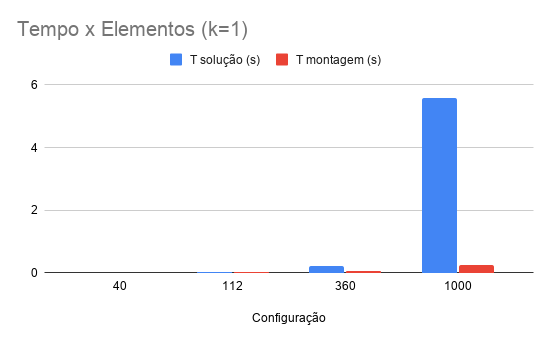
\includegraphics[width=\linewidth]{figuras/Capítulo 5/Parede estrutural/Tempo x Elementos (k=1).png}
      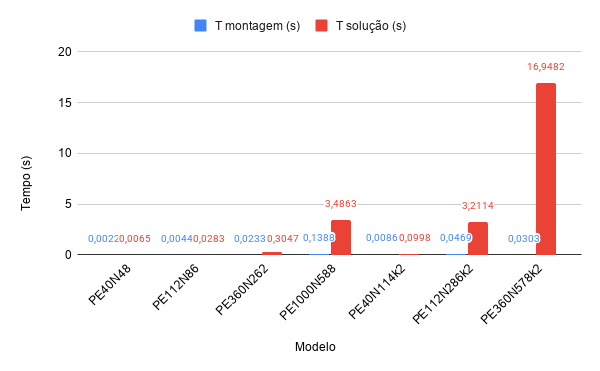
\includegraphics[width=\linewidth]{figuras/Capítulo 5/Parede estrutural/Tempo de montagem e solução comparação k.png}
    \end{column}
    \begin{column}{0.3\textwidth}
      \centering
      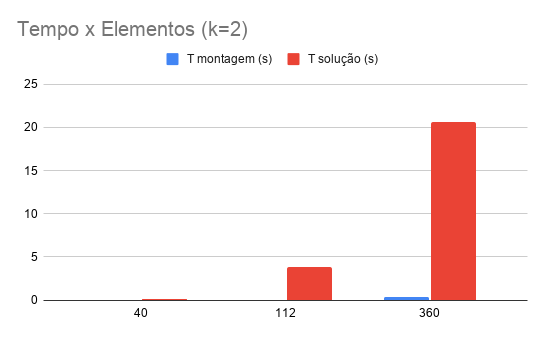
\includegraphics[width=\linewidth]{figuras/Capítulo 5/Parede estrutural/Tempo x Elementos (k=2).png}
      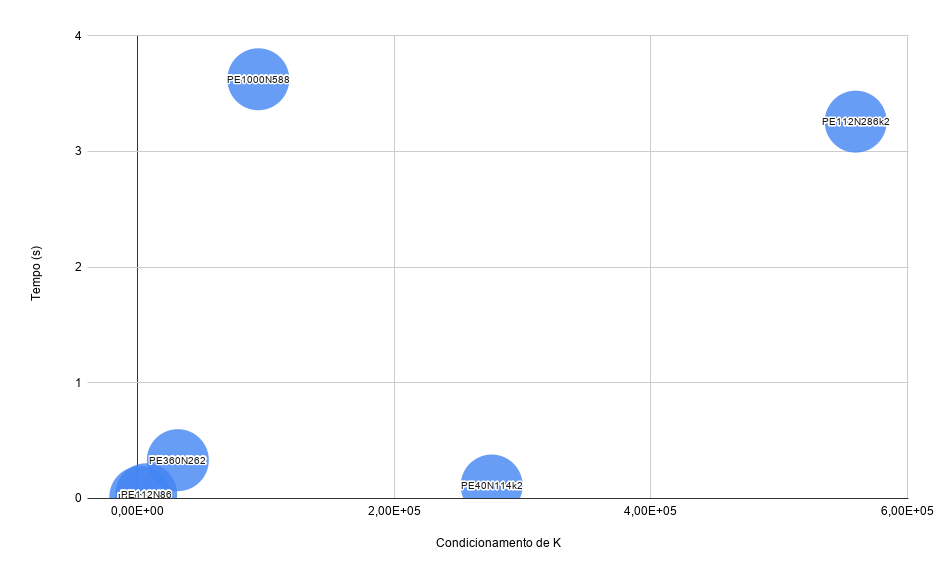
\includegraphics[width=\linewidth]{figuras/Capítulo 5/Parede estrutural/TxCond - K.png}
    \end{column}
    \begin{column}{0.3\textwidth}
      \centering
      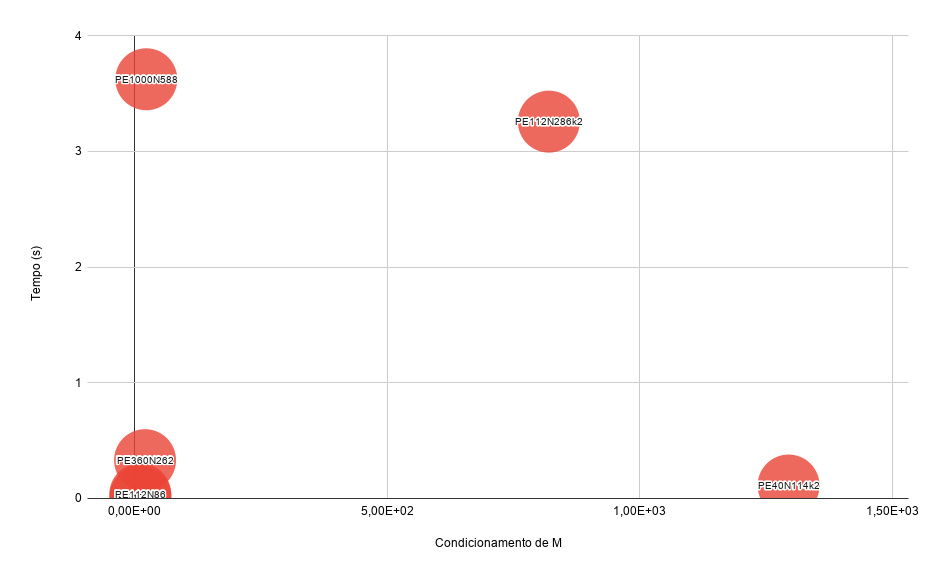
\includegraphics[width=\linewidth]{figuras/Capítulo 5/Parede estrutural/TxCond - M.png}
      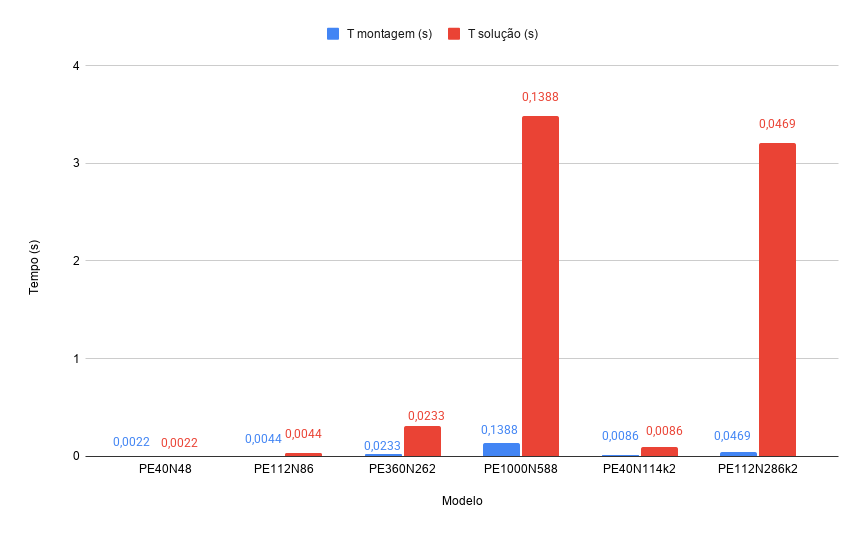
\includegraphics[width=\linewidth]{figuras/Capítulo 5/Parede estrutural/TxElementos.png}
    \end{column}
  \end{columns}
\end{frame}

\section{Discussão e conclusões}

\begin{frame}{Discussão consolidada}
  \begin{itemize}
    \item O MEV é competitivo (e em vários cenários superior) quando a malha é equilibrada.
    \item A estabilização é o ponto mais sensível da formulação.
    \item Bases polinomiais monomiais escaladas mostram limitações em alta ordem e elementos distorcidos.
    \item Flexibilidade geométrica do MEV é vantagem real para contornos complexos (furos).
    \item Em vibração livre não amortecida, a estabilização de massa pode ser anulada com ganho de precisão.
    \item Custo computacional e condicionamento precisam ser monitorados.
  \end{itemize}
\end{frame}

\begin{frame}{Principais conclusões}
  \begin{enumerate}
    \item Formulação do MEV para vibração livre em estado plano implementada e validada com sucesso.
    \item Malhas poligonais grosseiras, porém equilibradas, podem rivalizar com malhas clássicas refinadas.
    \item Estabilização de massa pode (e frequentemente deve) ser anulada em problemas espectrais não amortecidos.
    \item Parâmetro de estabilização da rigidez e escolha da base polinomial são críticos.
    \item Em configurações adequadas o MEV iguala ou supera o MEFG nas métricas globais.
  \end{enumerate}
\end{frame}

\begin{frame}{Perspectivas e trabalhos futuros}
  \begin{itemize}
    \item Investigação de bases polinomiais alternativas (ortogonais, serendipity).
    \item Formulações livres de estabilização ou com parâmetros adaptativos.
    \item Elementos virtuais com arestas curvas.
    \item Extensão para 3D, grandes deformações e problemas enriquecidos (X-VEM).
    \item Análise de dispersão e estabilidade para integração no tempo.
  \end{itemize}
\end{frame}

\begin{frame}{Agradecimentos}
  \begin{itemize}
    \item Ao orientador Prof.\ Dr.\ Marcos Arndt, pelo acompanhamento e discussões.
    \item Ao PPGMNE e à Universidade Federal do Paraná.
    \item Aos colegas e pesquisadores cujos trabalhos anteriores em MEF e MEFG forneceram a base de comparação (Torii, Cittadin, Custódio).
    \item À banca examinadora, pela disponibilidade e tempo dedicado.
  \end{itemize}
\end{frame}

%=============================================================================
\begin{frame}
  \centering
  \vspace{1.5cm}
  {\LARGE\bfseries Obrigado}

  \vspace{0.8cm}
  {\large Perguntas e discussão}

  \vspace{1.8cm}
  Vinícius Belmar Almeida Prado Pohl\\[0.3em]
  PPGMNE $\cdot$ UFPR $\cdot$ 2026
\end{frame}

} % fim do usebackgroundtemplate

\end{document}